\documentclass[12pt]{article}

\usepackage{fullpage}
\usepackage{multicol,multirow}
\usepackage{tabularx}
\usepackage{ulem}
\usepackage[utf8]{inputenc}
\usepackage[russian]{babel}
\textheight=24cm
\usepackage[pdftex]{graphicx}
\graphicspath{{pictures/}}
\DeclareGraphicsExtensions{.pdf,.png,.jpg}

\begin{document}

\section*{Лабораторная работа №\,3 по курсу дискретного анализа: Исследование качества программ}

Выполнил студент группы 08-207 МАИ \textit{Лебедев Иван}.

\subsection*{Условие}

\begin{enumerate}
\item Для реализации словаря из предыдущей лабораторной работы, необходимо провести исследование скорости выполнения и потребления оперативной памяти. В случае выявления ошибок или явных недочётов, требуется их исправить.

\end{enumerate}

\subsection*{Дневник отладки}

\par \textbf{1. gprof}
\par Для профиляции программы утилитой gprof необходимо скомпилировать её с флагом -pg, затем запустить исполняемый файл с какими- либо тестами, в результате чего создаётся файл gmon.out с данными о времени работы функций программы. Эти данные можно представить в виде таблицы с помощью самой утилиты gprof.
\par На тестах в 200 000 строк я получаются следующие результаты: 

\noindent 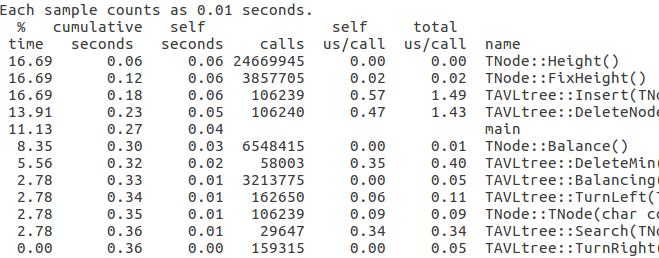
\includegraphics{200k}

Если запустить программу с тестом в 400 000 строк то результаты будут следующими:

\noindent 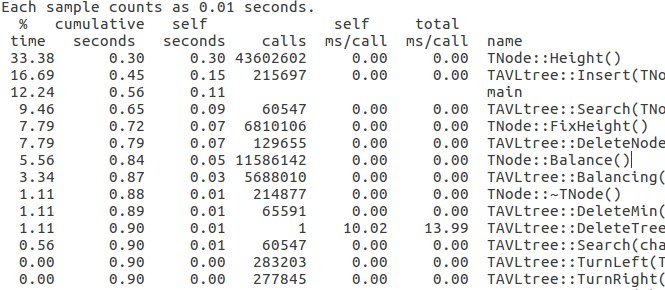
\includegraphics{400k}

По этим данным можно понять, что больше всего времени занимает функция Height(), а также Insert() и Search().

\par \textbf{2. valgrind}
\par Valgrind - программное обеспечение, предназначенное для отладки использования памяти, обнаружения утечек памяти. Программа запускается с помощью valgrind --leak-check=full --show-leak-kinds=all, и подаются на вход тесты. В результате работы программы можно видеть, что вся выделенная память очищается, и нет утечек и ошибок памяти.

\noindent 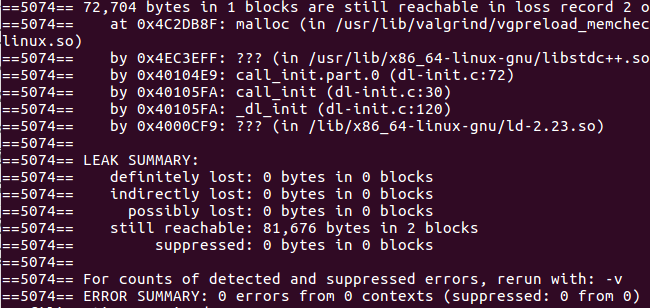
\includegraphics{valgrind}

\subsection*{Выводы}

Утилитой gprof можно выявить места в программе в которых она работает дольше всего, и точечно ускорить её, тем самым не тратя время на и так быстрые функции.
Утилитой valgrind можно узнать об утечках памяти, об освобождении уже освобожденной памяти и многих других ошибках. Что упрощает нахождение множества ошибок.

\end{document}

